\chapter{Background}

\section{Introduction to Research Area}

The maximum observed sea level extreme in Trondheim is 2.06m (NN2000), recorded in 1971. Trondheim municipality plans indicate the city should be prepared for 4.87m by 2100. 

Trondheim is situated in a protected location, deep within Trondheimsfjord. This protected location combined with the geological setting means that the assumption could be that Trondheim is not a risk from sea level extremes. This is further exaggerated by the understanding that Norwegian land is rising due to glacial melt. However, isostatic uplift is an incredibly varied process across the country and the basic model that the majority of the population has about sea level rise and land rise, may be creating a false confidence. 



Locations of Project Background
Maps here
Places chosen to research 

Trondheim and SlEs
•	2.06 m high water (NN2000)
•	Maximum observed in Trondheim is 2.60m in 1971
•	City plans for 4.87m by 2100
•	More details on chosen research areas
•	Include maps here 
•	Social demographic stats
•	Risk level stats

\section{Research Sites}
Four sites which are situated on Trondheims coast were chosen to represent the resilience for the city. These locations were chosen for their high daily population throughput and large amounts of infrastructure. The physical vulnerability to sea level extremes is diverse for these sites as can be seen in figure** below and is further outlined in table** below. 
\paragraph{}
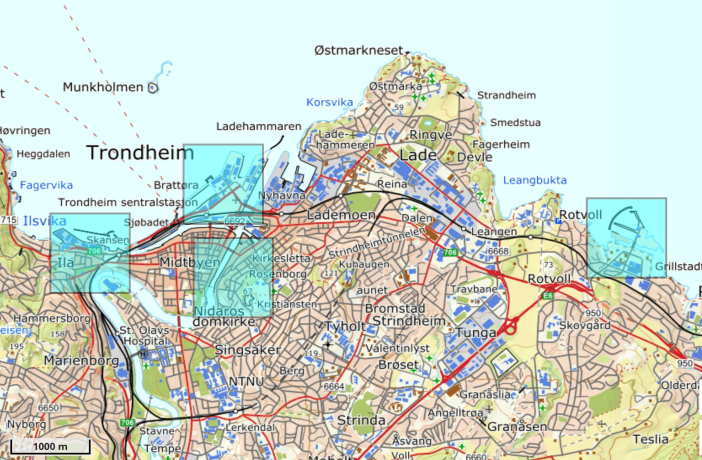
\includegraphics[width=0.9\textwidth]{fig/map of chosen areas.png}
*i can do this map better and include - scale, north, positioning relative to Norway etc, but this will do for just now*
\paragraph{}

Four research sites were selected based on coastal characteristics, infrastructure and high levels of daily population. Factors included in physical vulnerability are natural resistance to erosion, engineered resistance to erosion, engineered protection to sea level extremes, infrastructure directly upon coastline, settlements patterns, usage patterns and projected changes in sea level extremes. The four sites selected were Brattøra, Nidelva, Skansen and Grillstad. The physical vulnerability was determined from direct observation, kvartverket models and consulting planning documents (TEK10 /17) for each site. \cite{miljoenheten_og_byplankontoret_trondheim_kommune_9-notat-om-havnivastigning-og-stormflo---hensyn-i-arealplanlegging-nyhavnapdf_2020}


\paragraph{}
\begin{table}[!ht]
    \centering
    \begin{tabular}{|l|l|l|l|l|}
    \hline
        location & Brattøra & Grillstad & Skansen  & Nidelva \\ \hline
        PV 70 years ago & high & high & medium & Low \\ \hline
        PV now &  medium &  medium &  low &  low \\ \hline
        PV in 70 years &  high &  high &  medium &  medium \\ \hline
        Dominant & Office space  & Residential & Recreational  & Residential and \\ \newline
        use & and harbour &  only   &  and industry & and commercial  \\ \hline
        Land type & Reclaimed land & Reclaimed land & Managed coastline  & Altered tidal river \\ \hline
        protection & Harbour wall & Harbour wall & Harbour wall, placed rocks & inland \\ \hline
    \end{tabular}
    \caption{Research Sites PV = physical vulnerability to the sea}
    \label{table:research-sites}
\end{table}

Brattøra is the research site with the least amount of residential population. The dominant use is as office space, which is protected by a harbour wall and a small harbour behind that. The location is upon reclaimed land and for this reason it has very high physical vulnerability 70 years ago. The modern day harbour and areas design allows it to have medium physical vulnerability now, but it is projected to have several sections regularly flooded in 70 years. Currently these areas are predominantly sustainable urban development schemes with footpaths and car parks where a lot of the flooding would occur, but there is still risk of more significant impacts from sea level extremes beyond nuisance flooding, shutting off of important transport routes and preventing access to offices.
\paragraph{}
Grillstad is also located on reclaimed land and again has very high physical vulnerability 70 years ago. It is also located behind a harbour and harbour wall, in contrast to  Brattøra the dominant use is residential. There is several small commercial ventures, but the vast majority are their to serve the needs only of local residents. There is no major transport connections or industry in this sites. 
\paragraph{}
Nidelva is a less obvious choice for research into sea level extremes as it is situated further from the coastline. The land type here is altered tidal river and its physical vulnerability 70 years ago is low. The dominant use is residential and commercial and it has lower physical vulnerability predicted in 70 years than Brattøra and Grillstad. Nidelva site has the added complication of the river level potentially impacting the height of the water at certain times. The river here is controlled by the damn in....
\paragraph{}
Skansen has two dominant uses of recreational and industry. However there is also significant residency in the area, the majority being high rise flats at least ***check** 100m from the coastline. While several aspects of this coastline may appear more natural it is a managed coastline which is protected by placed rocks, a harbour wall and small bays. 
\paragraph{}


\section{Communication Design}
guidelines used for survey design

guidelines used for advertising

guidelines used for visual communication

guidelines used for communication about climate change
\paragraph{}

When utilising citizen science communication styles is very important. This section details the various methods used to reach subjects and encourage them to participate. Accessibility, trust and legitimacy are important attributes with all citizen science, but even more so in subjects with a potential emotional impact. A simulated image which shows a place a participant cares about as being impacted by a sea level extreme could result in a strong emotional impact which if not handled carefully could turn the participant away from the survey and research on this in general.
\paragraph{}
The Web Accessibility Guidelines and Story Map Accessible Design Principles were actively used during the creation of the website and online surveys. These guide good standard of visual communication. The guidline used for text  was the Principles for effective communication and public engagement on	climate change: A Handbook for IPCC authors. While not written for citizen science its advice for when discussing climate change and how to connect with people on these subjects was very useful. 
\paragraph{}
The design principles which were followed can be summarised as:
\begin{itemize}
    \item Make it as easy as possible to participate
    \item Utilize personal brand to enhance connection and trust
    \item Be succinct
\end{itemize}
\paragraph{}
These were created on from the guidelines mentioned above plus previous experience working in communications as well as training in visual communication, particularly cartography. To enhance legitimacy the results of this project will be shared to interested subjects via the website which was created to reach subjects after completion. 
\paragraph{}
In the appendix you can find example emails, social media posts and the poster used to access subjects. The full survey in Norwegian and English is also attached to demonstrate how the communication guidelines used were implemented.
\paragraph{}

o	 I used 2 sites 
%https://storymaps.arcgis.com/collections/d34681ac0d1a417894a3a3d955c6913f?item=15 story map accessible design principles 
%https://www.w3.org/WAI/standards-guidelines/wcag/ Web Content Accessibility Guidelines (WCAG)
Plus experience in coms and map design
Which highlights succinct is king
•	Communication style guideline used
Corner, A., Shaw, C. and Clarke, J. (2018). Principles for effective communication and public engagement on
o	climate change: A Handbook for IPCC authors. Oxford: Climate Outreach 


%decisions dont go here, but in the methods